\chapter{Background and Related Work}
\label{chap:background}

This chapter provides a comprehensive introduction to the theoretical framework and key concepts that underlie the research presented in this thesis. It begins by establishing the foundational knowledge necessary to understand the scope and objectives of the study. Following this, the chapter systematically examines fundamental principles related to deep learning and computer vision, offering a structured overview of essential methodologies and techniques. As the discussion progresses, more complex aspects of computer vision are explored, culminating in a review of previous research in the domain of computer vision.

\section{Football analytics}
\label{sec:football_analytics}

\subsection{Common analysis}

Football is a continuous game, as opposed to the discrete nature of more solved games like cricket, baseball or basketball. If we look at baseball, it has clear well defined actions with an beginning and an end. After an action in football, lets say a pass from the goalkeeper to a defender, the game does not stop. The defender keeps on playing. This creates an unfathomable number of possible permutations for each play. This hinders the current possible models from creating a complete understanding for type of play within football. 
\begin{displayquote} We're increasingly convinced that there's a lack of data that provides real information about the things that make you successful in football -Christofer Clemens, head analyst for Germanys national team in 2014 \end{displayquote}

One of the most insightful metrics for football analysis is the \acrfull{xg}. Introduced on April 9th 2012 (https://www.statsperform.com/resource/assessing-the-performance-of-premier-league-goalscorers/), most clubs, broadcasters and fans have adopted the metric. The metric exists because football is a low-scoring game, where the score might not always reflect the "felt nature" of the game. Expected goals measures the quality of a chance. The model which predicts \acrshort{xg} is a machine learning approach using \textbf{XGBOOST}. There is a database owned by Opta containing 1 million shots which is used. 

Most individual statistics are measured using GPS vests. The vests measure hearth rate and relative position on the pitch. Distance run, top speed and acceleration helps physiotherapists determine the physical conditions of the players. The data gives signs for injury detection, but it does not provide any tactical insight. Neither does it provide data for the opposing team or the ball. 

Team statistics in football are manual labor. Statistics like shots, shots on target, corners, free-kicks, possession etc. are manually annotated. This is a costly process, and a club like \acrshort{rbk} buys this data from a third party. This levels out the playing field because everyone has access to the same data, if they pay a handsome sum. 

Liverpool and more recently Arsenal in the Premier League has achieved good success with corner analytics using Deep Learning. A corner is a discrete event. The action has a deterministic start and end, which creates an opportunity to do end-to-end analysis. Cite the liverpool papers

\section{Deep Learning}
\label{sec:deep_learning}
Deep learning refers to a family of machine-learning techniques that construct models with multiple processing layers, designed to learn data representations with increasing levels of abstraction. Instead of relying on hand-engineered features, these methods automatically discover intricate structures directly from raw data. In early approaches, practitioners needed to carefully craft feature extractors to capture relevant information from inputs such as pixel intensities in an image. Deep learning, by contrast, uses layered architectures to progressively transform these raw inputs into representations that are well suited for tasks like detection and classification.\cite{lecun_deep_learning_2015}. 

In a deep neural network, early layers often learn simple features, such as edges or textures. Deeper layers combine these features to form parts or objects. The process is possible because of non-linear transformations that transform the input space. The transformations are parameterized by weights that are optimized through the backpropagation algorithm. By propagating error gradients backward through the network, the learning process adjusts millions of parameters to minimize discrepancies between the network’s predictions and the actual outcomes. This allows networks to learn complex functions from data, rather than manually defined rules. \cite{sanderson_deep_learning_2024}. 


\begin{align}
    \label{eq:forward_pass_b}
    y_l &= f(z_l) \\
    z_l &= \sum w_{kl} y_k \notag\\
    k\  &\epsilon\ Hidden\ units-H2 \notag
\end{align}
\begin{align}
    y_k &= f(z_k) \\
    z_k &= \sum w_{jk} y_j \notag\\
    j\  &\epsilon\ Hidden\ units-H1 \notag
\end{align}
\begin{align}
    \label{eq:forward_pass_e}
    y_j &= f(z_j) \\
    z_j &= \sum w_{ij} y_i \notag\\
    i\  &\epsilon\ Input \notag
\end{align}
    
\begin{figure}
    \centering
    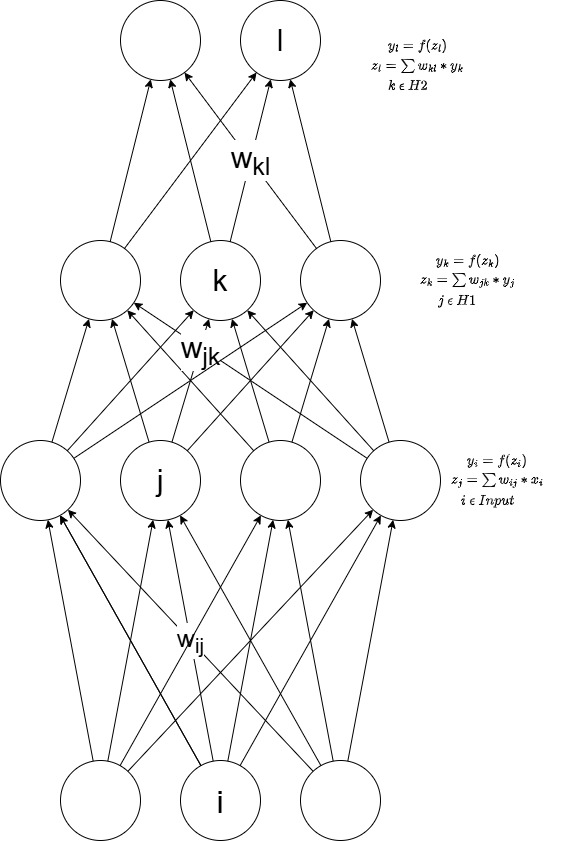
\includegraphics[width=0.5\linewidth]{figures/neural_net.jpg}
    \caption{\autoref{eq:forward_pass_b} through \autoref{eq:forward_pass_e} shows the equations used for a forward pass with two hidden layers. The bias term is ignored for simplicity. For every layer the total input \textit{z} is computed as a weighted sum of the layer below. \textit{f(.)} is applied to \textit{z} to get the final output.}
    \label{fig:multilayer_neural_net}
\end{figure}


\begin{align}
    \label{eq:backward_pass_b}
    \frac{\delta E}{\delta y_l} &= y_l-t_l \\
    \frac{\delta E}{\delta z_l} &= \frac{\delta E}{\delta y_l} \frac{\delta y_l}{\delta z_l} \notag
\end{align}

\begin{align}
    \label{eq:backward_pass_m}
    \frac{\delta E}{\delta y_k} &= \sum_{l\ \epsilon\ out} w_{kl} \frac{\delta E}{\delta z_l} \\
    \frac{\delta E}{\delta z_k} &= \frac{\delta E}{\delta y_k} \frac{\delta y_k}{\delta z_k} \notag
\end{align}

\begin{align}
    \label{eq:backward_pass_e}
    \frac{\delta E}{\delta y_j} &= \sum_{k\ \epsilon\ H2} w_{jk} \frac{\delta E}{\delta z_k} \\
    \frac{\delta E}{\delta z_j} &= \frac{\delta E}{\delta y_j} \frac{\delta y_j}{\delta z_j} \notag
\end{align}

\begin{figure}
    \centering
    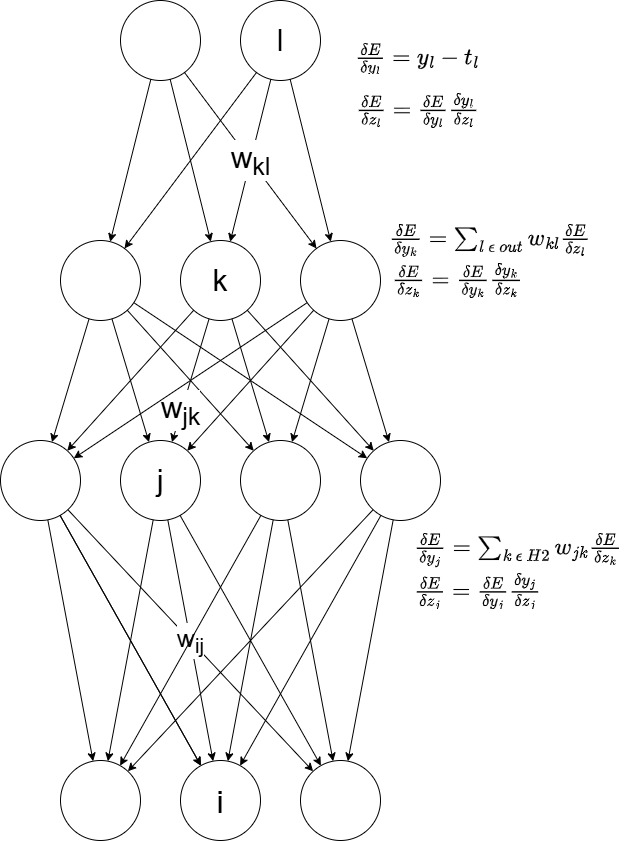
\includegraphics[width=0.5\linewidth]{figures/neural_net_back_prop.jpg}
    \caption{\autoref{eq:forward_pass_b} through \autoref{eq:forward_pass_e} shows the equations used for a forward pass with two hidden layers. The bias term is ignored for simplicity. For every layer the total input \textit{z} is computed as a weighted sum of the layer below. \textit{f(.)} is applied to \textit{z} to get the final output.}
    \label{fig:multilayer_neural_net}
\end{figure}


The equations \autoref{eq:backward_pass_b}, \autoref{eq:backward_pass_m} and \autoref{eq:backward_pass_e} computes the backward pass. The process begins by determining the error gradient for each output unit directly from the cost function. For instance, if the cost function for unit \textit{l} is defined as \(0.5(y_l-t_l)^2\) (where \(t_l\) is the target value), differentiating with respect to \(y_l\) yields an error term of \(y_l-t_l\).

For a hidden unit, the error gradient with respect to its output is not obtained directly. Each hidden unit’s output error is the accumulation of the gradients coming from the next layer, with each gradient scaled by the weight connecting the hidden unit to that future unit. After this aggregation, the error derivative relative to the unit’s output is "pushed back" to determine the error with respect to its input. This is achieved by multiplying the error derivative by the derivative of the activation function \textit{f(z)}. This operation converts the error derivative from the output space to the input space of the activation function.

Once the error derivative with respect to the pre-activation input (denoted as \(\frac{\delta E}{\delta z_k}\)) is calculated for a given unit in the current layer, the gradient for any weight \(w_{jk}\)—linking unit j in the previous layer to unit \textit{k}—is computed straightforwardly. It is given by multiplying the activation \(y_j\) from the previous layer by the error gradient \(\frac{\delta E}{\delta z_k}\). This product, \(y_j \frac{\delta E}{\delta z_k}\), tells us how much the weight contributes to the overall error, guiding how the weight should be adjusted during training.

\subsection{Convolutions}

Convolutions process structured multi-array data. An RGB image is naturally represented as three two-dimensional arrays corresponding to the red, green and blue channel. One dimensional arrays, audio or text, and three dimensional arrays for volumetric or videos use the same principles. \acrlong{cnn}s use local connectivity, pooling operations, shared weights and layering to exploit the properties and variances of natural signals. 

A typical \acrlong{cnn} is organized into multiple stages. The early stages consists of convolutional pooling layers. In a convolutional layer, each neuron connects to a local patch of inputs from the input or preceding layer through a filter of weights. The result of this weight summation is passed through an activation function. Pooling layers aggregate the nearby feature responses to reduce the spatial resolution. Stacking these layers incrementally builds more and more abstract representations of the data\cite{lecun_deep_learning_2015}. 

A turning point for \acrshort{cnn}s was in 2012 with the introduction of \textbf{AlexNet}\cite{krizhevsky_alexnet}. AlexNet revolutionized image classification tasks and sparked an interest in the subject of \acrshort{cnn}s. In the context of video classification the challenge extends from the spatial to the spatiotemporal dimension. \textbf{DeepVideo} \cite{karpathy_deep_video}(2014) extends convolutional operations into the time domain. \textcite{tran_2_plus_1_convolution} introduced the concept of \textbf{(2+1)D} convolutions. The poor scaling of normal 3D convolutions motivated a solution which consists of decomposing the convolutions into the spatial and temporal dimension. The \textbf{inflated 3D \acrlong{cnn}}(I3D)\cite{carreira_2017_i3d_quo_vadis} uses pretrained 2D convolutional weights and inflates them to the temporal dimension. I3Ds offer a balance between computational efficiency and representational power. Despite the inherit limitation of \acrshort{cnn}s to capture long-range temporal dependencies, the I3Ds have established themselves are key components in modern frameworks\cite{bhogal_human_2023} \cite{maheriya__2024_aerial_cnn}.


\subsection{Recurrent Neural Nets}

\acrfull{rnn} is useful for working with sequential data, but their vanishing gradient hinder them from being useful on their own. \acrfull{lstm} is the first solution to this problem \cite{bhogal_human_2023} \cite{kumar_human_2023} \cite{mahaseni_spotting_2021}. \acrshort{lstm}s address the vanishing gradient by providing a memory to the models, which help maintain temporal information. 
Because \acrshort{lstm}s have multiple input, forget and output gates their parameter count and computational complexity increases quickly. The structure can lead to overfitting on small datasets.  

The other widespread solution is the \acrfull{gru} \cite{giveki_human_2024} \cite{li_oarnet_2024} \cite{yu_i3d_2023}. \acrlong{gru}s use a reset gate and an update gate to maintain or discard information. It has fewer parameters than an \acrshort{lstm} which makes it an interesting alternative\cite{survey_of_survey}.

\subsection{Vision transformers}

Transformers had their breakthrough in 2017 with the paper \textit{Attention is all you need}\cite{vaswani_attention_2017}, and as they say; \textit{The rest is history}. ChatGPT later brought the transformer to the center of the internet, proving its effectivity in \acrfull{nlp}. $25.5\%$ of the articles included in the "full-text screening" contained the word transformer, contrasting to $8.5\%$ which had the word \textit{recurrent} or $14.9\%$ with the word \textit{convolution}. The transformer is the most important approach to action spotting and activity recognition. 

TimeSformer \cite{bertasius_timesformer_2021} is based on a \acrfull{vit} adapted to the video domain. The \acrlong{vit} decomposes images into patches. The TimeSformer decomposes a video into patches both in the temporal and spatial dimension. The VViT \cite{arnab_vvit_2021} achieved \acrlong{sota} in several categories on Papers with Code when it was released in 2021. 

The novel \acrlong{sam} from Meta employs transformers. The winning contribution of last years SoccerNet action spotting challenge \cite{denize_comedian_2024} utilizes transformers. \cite{sarraf_optimal_2023} studies the challenges of transformers towards real-time action recognition with good success. 

Vision transformers achieve success, but they can struggle when there is a lack of training data. They are also prone to high model complexity, long training times and large models \cite{lee_enhancing_mamba_s6_2024}.


\section{Action Recognition Techniques} 
\label{sec:action_recognition_techniques}

\subsection{Hand-Crafted methods}

As is common in the domain of computer vision, hand-crafted methods were the most influential before deep learning arrived. The histogram of gradients\cite{dalal_histogram_of_gradients} and histogram of flow \cite{dalal_histogram_of_flow} are early solutions to the action recognition problem. The histogram of gradients is designed to spot humans in static images, by dividing an image into patches. Between the patches, gradients are calculated to create a vector description. The histogram-of-flow is based on optical flows and is used in videos. A histogram of gradient vector is made at each frame, and the relation between the frames is saved in a descriptor and used to analyze. 

The issues from hand crafted methods has become evident with the rise of deep learning. Complex scenarios, scaling and poor generalization limit the usefulness of the hand-crafted methods. 

\subsection{Masking}

Encoding and masking techniques are used with video data because of their unavoidable large size. Encoding encapsulates the process of compressing video files to reduce size while keeping a satisfactory quality. Video masking is the technique used to discard uninteresting regions and patches to focus on more meaningful features. This motivates the model to learn meaningful representations, rather than predicting based on redundant data \cite{tong_videomae_2022}. The most prominent masking variant used on \acrshort{sota} benchmarks on Papers with Code' in the category \textit{Action Recognition}\footnote{\url{https://paperswithcode.com/task/action-recognition-in-videos}} is the VideoMAE V2 \cite{wang_videomae_2023}. 

Tong et al. \cite{tong_videomae_2022} address the problem of training video transformers from scratch. The aim is to use self-supervised learning to capture meaningful representations which enables the model to decode data into the original representations. The contributions of the masked autoencoder \cite{tong_videomae_2022} are the ability to train \acrshort{vit}s on smaller datasets. VideoMAE \cite{tong_videomae_2022} also tackle the problems of temporal relations in video-data and suggests a high masking ratio. VideoMAE-V2 \cite{wang_videomae_2023} improves the VideoMAE-models training time. It is still a very computationally expensive approach. 


\subsection{Knowledge Distillation}

Knowledge distillation \cite{denize_comedian_2024} \cite{li_videomamba_2024} \cite{bose_soccerkdnet_2023} is the technique where a smaller and simpler student-model learns to replicate the performance of a more advanced and complex teacher-model without learning all the concepts. This is a valuable method because of the computational requirements of video processing. The method provides a way to make a smaller more manageable model. The student-model is evaluated against the teacher to find a trade-off between complexity and accuracy. 

If the teacher model is not of sufficient quality, knowledge distillation is an ineffective approach. The training of several different student models has a significant computational cost. The loss of complex relations from the teacher to the student can make the student less able to generalize across different domains.


\subsection{Bi-Directional layers}

Bi-directional layers process data both in the forwards and backwards direction in a model. A Bi-\acrshort{lstm} model \cite{radhakrishnan_bi_lstm_2023} \cite{bhogal_human_2023} consists of two \acrshort{lstm} layers. One predicts the sequence from start to finish while the others processes the data from finish to start. If one imagines how much a football field changes after a goal, compared to before a goal, this is a intuitive approach to model it better. A bi-directional layer leads to longer training time and larger computational demands. 


\subsection{Skeleton and Posture Estimation}

Skeleton and posture estimation \cite{elaoud_skeleton-based_2020} \cite{wang_skeleton_two-stream_2023} \cite{reilly__skeleton_just_pi_2023} aims to detect joints in the human body. The methods use the relations between joints to interpret motion patterns. Skeleton-based models struggle when the entities are occluded, which is often the case in football.

\section{Applications in Football}
\label{sec:applications_in_football}

COMEDIAN \cite{denize_comedian_2024} combines self-supervised learning and knowledge distillation to initialize a transformer for action-spotting on the SoccerNet-V2 dataset \cite{deliege_soccernet-v2_dataset_2021}. The contributions from Denize et al. are a three-step training pipeline and \acrshort{sota} performance. The first step is to use self-supervised pretraining on a spatial transformer. The second step is to initialize a temporal transformer by using knowledge distillation to enrich the spatial transformers output. The last step is the training on the relevant action spotting task, in this case the SoccerNet-V2 \cite{deliege_soccernet-v2_dataset_2021}.

T-DEED \cite{xarles_t-deed_2024} is a Temporal-Discriminability Enhancer Encoder-Decoder, which won the action spotting category of SoccerNet 2024 \cite{cioppa_soccernet_2024}. The temporal part refers to looking at different lengths of time in the video. Discriminability is making sure each frame of the video is distinct. Encoder-decoder refers to compressing and expanding the video information. The model utilizes \acrfull{sgp} to enhance its discriminability between tokens. This is useful because sports actions can appear similar. 

In 2021 Gerats et al. \cite{gerats_individual_same_task_2021} worked with a single static panorama camera for action-spotting and activity recognition. They use player snippets as model input. Inflated 3D \acrshort{cnn} is used to extract spatio-temporal features from the snippets. A graph attention network is used to analyze the relationship between players and their activities and actions. 

% \section{Challenges}
% \label{sec:challenges}

% The masked autoencoder \cite{tong_videomae_2022} is very computationally expensive, requiring 64 A100 GPUs for 14 days to train \cite{wang_videomae_2023}. Video data is inherently expensive to work with and requires powerful GPUs to work with. This prevents widespread research and equal opportunities to work on it \cite{survey_of_survey}. 

% The similarity between image processing and video processing is not mirrored in the size of their datasets. Thorough surveys \cite{survey_of_survey} \cite{seweryn_survey_2023} of both activity recognition in general and it's application in football point to the lack of annotated datasets to achieve similar performances to image benchmarks. Meta \cite{ravi_sam_nodate} claims a model which understands images must understand video. \cite{carreira_2017_i3d_quo_vadis} approach takes advantage of convolutional kernels pre-trained on images. Their performance on video data is poorer than on images. 


\section{Technological Advances}
\label{sec:technological_advances}

\subsection{Mamba}
The \acrfull{s6} \cite{gu_mamba_2024} is a novel approach in the field of video analysis \cite{li_videomamba_2024}. A \acrlong{s6} is conceptually based on a continuous mapping from a 1-D function or sequence through a hidden state. \acrlong{s6}s implement the following

\[h'(t) = \textbf{A}h(t)+\textbf{B}x(t)\]
\[y(t) = \textbf{C}h(t)\]


\[h_t = \textbf{A}h_{t-1}+\textbf{B}x_t\]

\(x_t\) represents the input at time \(t\). In the case of action recognition, $x_t$ is a vector which describes the spatiotemporal features extracted using the % \todo{explain what the embedding step is?}
embedding step. The hidden state \(h_t\) at time step \(t\) is updated based on the previous hidden state \(h_{t-1}\) and the current input \(x_t\). The matrix \(\textbf{A}\) determines how \(h_{t-1}\), the memory from all previous steps affect the current hidden state \(h_t\). \(\textbf{B}\) determines how the current input affects the hidden state \(h_t\).

\[y_t = \textbf{C}h_t\]

$y_t$ is the output at time t. The matrix \(\textbf{C}\) calculates the output from the hidden state. 

\[\bar{\textbf{A}} = exp(\Delta\textbf{A)} \]
\[\bar{\textbf{B}} = exp(\Delta\textbf{A)}^{-1}(exp(\Delta\textbf{A)} - \mathbf{I}) * \textbf{B} \]

Mamba is a discrete state-space model, which implements a selective scan mechanism (S6) as its core operator. The \acrshort{s6} model has the parameters $(\Delta, {A, B, C})$. 
\(\Delta\) is the step size,  which is a learnable parameter that represents the resolution of the input. \(\bar{\textbf{A}}\) and \(\bar{\textbf{B}}\) are the discretized matrices of respectively matrix \(\textbf{A}\) and matrix \(\textbf{B}\). Matrix \textbf{A} produces the hidden state. 

The discrete representation of a state space model is described as follows. 
\[h_k = \bar{\textbf{A}}h_{k-1} + \bar{\textbf{B}}x_k\]
\[y_k = \textbf{C}h_k\]

The State Space Models are inherently time invariant. The matrices $(\textbf{A}, \textbf{B}, \textbf{C})$ are static by nature. This prevents the model from having content awareness. Unlike a Transformer which can attend at different parts of a input sequence, the State Space Models do not have content awareness. The State Space Models have an efficient small state of the history which is not that powerful, while the attention matrix of a Transformer is very large in comparison and much more powerful. Mamba aims for a small state with the power of an attention matrix. 

% \todo{is this the same as the text above the equations?} Mamba makes the matrices $(\textbf{B}, \textbf{C}, {\Delta})$ dependent on the input. Matrix $\textbf{A}$ does not change. The size of $\Delta$ results in the focus of the model, a small $\Delta$ uses the context more, while a grander $\Delta$ has a heavier focus on temporal features. 

The \acrlong{s6} attempts to solve the slow and computationally expensive inference time of transformers. At the same time it must not lag behind in training time, where the transformers can use parallelization. Mamba ends up scaling linearly in time and complexity \cite{lee_enhancing_mamba_s6_2024}, in contrast to the quadratic scaling of transformers. VideoMAMBA \cite{li_videomamba_2024} shows the competitive accuracy of a MAMBA-based model.

MAMBA models are complex to implement compared to the straightforward approach of \acrshort{cnn}s. Neither has MAMBA proved its efficiency in the spatial domain compared to the \acrshort{cnn}. Comparisons to a \acrlong{rnn}, MAMBAs static \textbf{A} matrix might limit its adaptability. A \acrshort{rnn}, just like the \acrshort{cnn}, is significantly easier to implement than MAMBA. MAMBA is a less explored option, which could limit its community size and availability of help and resources compared to other methods. 

\subsection{META Segment Anything Model 2}

The \acrfull{sam} is a foundation model designed with a user interface to provide promtable visual segmentation. \acrshort{sam} handles both images and videos, and treats images as a video with one frame. The model is transformer-based  with a memory attention module to process video frames sequentially. \acrshort{sam} takes mouse clicks as one of the inputs to the inference step. The dataset which Ravi et al. created, SA-V, is publicly available and much larger than previous segmentation datasets for videos. The \acrfull{sam} is a versatile model, and the strong performance on both image segmentation and video segmentation shows its robustness. 

\subsection{VideoMAE-V2}

The VideoMAE-V2 \cite{wang_videomae_2023} is an improvement to the VideoMAE to enhance its scalability and performance. VideoMAE-V2 introduces a dual masking strategy which improves training time compared to the original version. VideoMAE-V2 scales to train with billion-level parameters. The model also shows a grander versatility than the VideoMAE and verifies its success on a variety of downstream tasks. 

\section{Datasets}
\label{sec:datasets}

Yin et al. \cite{survey_of_survey} provides comprehensive tables over available datasets for action recognition in sports. Table 4 and Table 5 are specifically relevant. Seweryn et al. \cite{seweryn_survey_2023} provides an even more specified research related to the topic of football datasets. 

\subsection{SoccerNet}

Deliege et al. \cite{deliege_soccernet-v2_dataset_2021} provides the dataset \textbf{SoccerNet-V2}, which offers annotations for various video-analysis tasks related to football. The dataset includes 500 labels for action spotting. SoccerNet will host a competition for ball action spotting in 2025, featuring 12 ball events and associated team annotations. The dataset is available for download at HuggingFace\footnote{\url{https://huggingface.co/datasets/SoccerNet/SN-BAS-2025}}.

\subsection{UCF101}

The UCF101 dataset \cite{dataset:UCF101} is a widely used benchmark for human action recognition in video data. It consists of 13,320 videos from 101 action categories, collected from YouTube. The dataset provides a diverse range of actions, including sports, musical instruments, and human-object interactions, making it a valuable resource for training and evaluating action recognition models. The videos are annotated with action labels, and the dataset is split into training and testing sets to facilitate performance comparison across different models.

\subsection{THUMOS}

The THUMOS dataset \cite{dataset:thumos} is another significant benchmark for action recognition and temporal action detection. It includes two main components: THUMOS Challenge and THUMOS'14. The dataset contains videos from 20 action classes, with annotations for both action classification and temporal localization. The THUMOS Challenge encourages the development of algorithms that can accurately detect and classify actions within untrimmed videos, providing a realistic scenario for evaluating the performance of action recognition systems.

\subsection{RBK Video Data}

\acrfull{rbk} possesses a substantial amount of football video data. Annotations exist in \textit{.xml} format. The nature of annotation done within \acrshort{rbk} is different to the SoccerNet annotation, and appears more complex with more classes and combination of classes. The data will not be published because of the competitive disadvantage this entails.
% This data, collected from various matches and training sessions, represents a valuable resource for developing and testing action recognition models specific to football. Annotating this data could significantly enhance the accuracy and applicability of these models, providing insights into player performance, tactical analysis, and game strategy. Leveraging advanced annotation techniques and machine learning models, such as semi-supervised learning, could facilitate the efficient processing and utilization of this extensive video repository.




